\documentclass{tufte-book}
\input{preamble.tex}

% Book metadata
\title{Truchet}
\subtitle{$4\times4$ patterns with $90^{\circ}$ rotational symmetry}
\author[]{}
\publisher{}

\begin{document}

% Front matter
%\frontmatter

% r.1 blank page
%\blankpage


% r.3 full title page
\maketitle


% v.4 copyright page
\newpage
\begin{fullwidth}
~\vfill
\thispagestyle{empty}
\setlength{\parindent}{0pt}
\setlength{\parskip}{\baselineskip}

\par\textit{Current printing, \today}
\end{fullwidth}

\cleardoublepage

\chapter*{Introduction}

\noindent
Traditionally, Truchet tiles are square tiles that are divided by a diagonal line, and coloured with two colours with a different colour on either side of the diagonal. Each tile can be rotated to one of four positions. Patterns are formed by placing tiles next to each other, rotating individual tiles to create repeated motifs.
This booklet presents a complete listing of $4x4$ Truchet tile patterns with $90^{\circ}$ rotational symmetry ($256$ patterns). \marginnote{\centering\input{intro_generated_files/tileList2.gtex}} Treating these $4x4$ tile patterns as tiles themselves allows for larger decorative patterns to be constructed from them. For example, a uniform frieze made from a single $4x4$ tile can actually produce interesting secondary patterns which help illustrate some interesting relationships that exist among the tile patterns.  

\vspace{0.5cm}
\noindent
Each $4x4$
Truchet tile pattern with rotational symmetry has a core $2x2$ pattern in one of its quadrants that is rotated to produce the overall pattern. \marginnote{\centering\begin{tikzpicture}[node distance=-0.7em]
    \matrix (xA) [anchor=west]
    {% 
        \node(xA1) [draw,right,font=\Large, minimum width=3em,minimum height=3em,fill=lightgray,
        , fill opacity=0.2, text opacity=1] {b} ;  \\
        \node(xA2) [draw,right,font=\Large, minimum width=3em,minimum height=3em,fill=lightgray,
        , fill opacity=0.2, text opacity=1] {a} ;  \\
    };
    \matrix (xB) [right=of xA]
    {% 
        \node(xB1) [draw,right,font=\Large, minimum width=3em,minimum height=3em,fill=lightgray,
        , fill opacity=0.2, text opacity=1] {d} ;  \\
        \node(xB2) [draw,right,font=\Large, minimum width=3em,minimum height=3em,fill=lightgray,
        , fill opacity=0.2, text opacity=1] {c} ;  \\
        %\node(xB3) [draw,anchor=west,font=\Large, minimum width=3em,minimum height=3em] {c} ;  \\
    };
    \matrix (yA) [above=of xA]
    {% 
        \node(yA1) [rotate=-90,draw,right,font=\Large, minimum width=3em,minimum height=3em] {a} ;  \\
        \node(yA2) [rotate=-90,draw,right,font=\Large, minimum width=3em,minimum height=3em] {c} ;  \\
     };
     \matrix (yB) [above=of xB]
    {% 
        \node(yB1) [rotate=-90,draw,right,font=\Large, minimum width=3em,minimum height=3em] {b} ;  \\
        \node(yB2) [rotate=-90,draw,right,font=\Large, minimum width=3em,minimum height=3em] {d} ;  \\
     };
    \matrix (xC) [right=of xB]
    {% 
        \node(xC1) [rotate=90,draw,right,font=\Large, minimum width=3em,minimum height=3em] {d} ;  \\
        \node(xC2) [rotate=90,draw,right,font=\Large, minimum width=3em,minimum height=3em] {b} ;  \\
    };
    \matrix (yC) [right=of xC]
    {% 
        \node(yC1) [rotate=90,draw,right,font=\Large, minimum width=3em,minimum height=3em] {c} ;  \\
        \node(yC2) [rotate=90,draw,right,font=\Large, minimum width=3em,minimum height=3em] {a} ;  \\
    };
 \matrix (xD) [above=of xC]
    {% 
        \node(xD1) [rotate=180,draw,right,font=\Large, minimum width=3em,minimum height=3em] {c} ;  \\
        \node(xD2) [rotate=180,draw,right,font=\Large, minimum width=3em,minimum height=3em] {d} ;  \\
    };
    \matrix (yD) [right=of xD]
    {% 
        \node(yD1) [rotate=180,draw,right,font=\Large, minimum width=3em,minimum height=3em] {a} ;  \\
        \node(yD2) [rotate=180,draw,right,font=\Large, minimum width=3em,minimum height=3em] {b} ;  \\
    };
\end{tikzpicture}} In this booklet, the core pattern, or prototile, is assumed to be in the lower left. Each pattern can identified as a sequence of $4$ digits $(a,b,c,d)$, or more succinctly, $abcd$, that list the rotational positions of each tile in the lower left quadrant. This sequence $abcd$ will be referred to as the \textit{signature} of the tile pattern.

\vspace{2cm}

\begin{center}
{
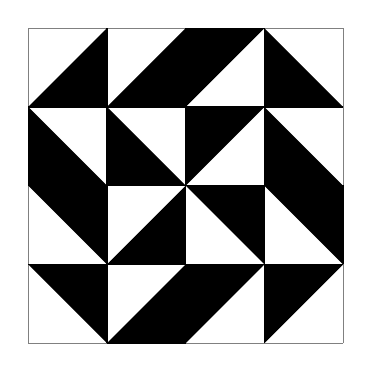
\begin{tikzpicture}[scale=1]
 \draw [step=1cm,gray,very thin](0,-1) grid (4,3); 
 \draw[opacity=1,fill=black](0,0)--(1,0)--(1,-1); 
 \draw[opacity=1,fill=black](0,1)--(1,1)--(1,0); 
 \draw[opacity=1,fill=black](1,1)--(0,1)--(0,2); 
 \draw[opacity=1,fill=black](1,3)--(1,2)--(0,2); 
 \draw[opacity=1,fill=black](2,0)--(2,-1)--(1,-1); 
 \draw[opacity=1,fill=black](2,1)--(2,0)--(1,0); 
 \draw[opacity=1,fill=black](2,1)--(1,1)--(1,2); 
 \draw[opacity=1,fill=black](2,3)--(2,2)--(1,2); 
 \draw[opacity=1,fill=black](2,-1)--(2,0)--(3,0); 
 \draw[opacity=1,fill=black](2,1)--(3,1)--(3,0); 
 \draw[opacity=1,fill=black](2,1)--(2,2)--(3,2); 
 \draw[opacity=1,fill=black](2,2)--(2,3)--(3,3); 
 \draw[opacity=1,fill=black](3,-1)--(3,0)--(4,0); 
 \draw[opacity=1,fill=black](3,1)--(4,1)--(4,0); 
 \draw[opacity=1,fill=black](4,1)--(3,1)--(3,2); 
 \draw[opacity=1,fill=black](4,2)--(3,2)--(3,3); 
\end{tikzpicture}

\textit{The 0011 pattern}
}
\end{center}

\chapter{Pattern families}

\noindent
We can group the $4x4$ Truchet tile patterns with rotational symmetry into families where  tile patterns are considered to be in the same family if they would look the same without colour -- if each corresponding tile shares the same diagonal direction. The sequence that represents the family of a tile pattern can be found by taking the sequence of the tile pattern \textit{modulo} $2$. So, for example, the $16$ tile patterns below are all members of the $0110$ family. 

\vspace{1.2cm}

\marginnote{\centering\input{ch1_generated_files/parent-0110.gtex}\\ \textit{The 0110 family pattern}}

{
\setlength{\tabcolsep}{3pt}
\renewcommand{\arraystretch}{2}
\input{intro_files/example_family}
{\begin{center} \textit{The 0110 pattern family}\end{center}}
}

\vspace{0.5cm}

\noindent
For a given family, there is corresponding \textit{companion} family, the family of patterns formed by rotating each square in a member of the original family by $90^{\circ}$.  There are also two \textit{skew} families, formed by taking the upper left and lower right quadrants of an original family tile pattern as a founding pattern and a \textit{dual} family, formed by taking the upper right quadrant as a founding patterns. A family is always different than its companion, and each family has a distinct companion, but it can happen that skew and duals can coincide. Self-dual families, where the dual family is the same as the original are of particular interest in the frieze patterns of the next chapter.

\section{Self-Dual families}
\input{ch1_generated_files/0000-relations.gtex}

\,
\newline
\vspace{1.2cm}
\input{ch1_generated_files/0110-relations.gtex}

\,
\newline
\vspace{1.2cm}
\input{ch1_generated_files/1001-relations.gtex}

\,
\newline
\vspace{1.2cm}
\input{ch1_generated_files/1111-relations.gtex}

\,
\newline
\vspace{1.2cm}


\section{Non self-dual families}
\input{ch1_generated_files/0001-relations.gtex}

\,
\newline
\vspace{1.2cm}
\input{ch1_generated_files/0010-relations.gtex}

\,
\newline
\vspace{1.2cm}
\input{ch1_generated_files/0011-relations.gtex}

\,
\newline
\vspace{1.2cm}
\input{ch1_generated_files/0100-relations.gtex}

\,
\newline
\vspace{1.2cm}
\input{ch1_generated_files/0101-relations.gtex}

\,
\newline
\vspace{1.2cm}
\input{ch1_generated_files/0111-relations.gtex}

\,
\newline
\vspace{1.2cm}
\input{ch1_generated_files/1000-relations.gtex}

\,
\newline
\vspace{1.2cm}
\input{ch1_generated_files/1010-relations.gtex}

\,
\newline
\vspace{1.2cm}
\input{ch1_generated_files/1011-relations.gtex}

\,
\newline
\vspace{1.2cm}
\input{ch1_generated_files/1100-relations.gtex}

\,
\newline
\vspace{1.2cm}
\input{ch1_generated_files/1101-relations.gtex}

\,
\newline
\vspace{1.2cm}
\input{ch1_generated_files/1110-relations.gtex}

\,
\newline
\vspace{1.2cm}


\section{Family and tile pattern mappings}

\marginnote{\centering\input{intro_generated_files/tileList2.gtex}} 
Related families and tiles can be obtained from applying simple mappings on the signature of the tile pattern.

\subsection{Family mappings}
\begin{align*}        \text{companion}: (a,b,c,d) &\mapsto (a+1, b+1, c+ 1, d+1) \pmod{2};\\
    \text{skew}+ : (a,b,c,d) &\mapsto (c+1, a+1, d+ 1, b+1) \pmod{2};\\
    \text{reverse} : (a,b,c,d) &\mapsto (d, c, b, a) \pmod{2};\\
    \text{skew}- : (a,b,c,d) &\mapsto (b+1, d+1, a+ 1, c+1) \pmod{2};
\end{align*}

\subsection{Tile pattern mappings}
\marginnote{\centering\begin{tikzpicture}[node distance=-0.7em]
    \matrix (xA) [anchor=west]
    {% 
        \node(xA1) [draw,right,font=\Large, minimum width=3em,minimum height=3em,fill=lightgray,
        , fill opacity=0.2, text opacity=1] {b} ;  \\
        \node(xA2) [draw,right,font=\Large, minimum width=3em,minimum height=3em,fill=lightgray,
        , fill opacity=0.2, text opacity=1] {a} ;  \\
    };
    \matrix (xB) [right=of xA]
    {% 
        \node(xB1) [draw,right,font=\Large, minimum width=3em,minimum height=3em,fill=lightgray,
        , fill opacity=0.2, text opacity=1] {d} ;  \\
        \node(xB2) [draw,right,font=\Large, minimum width=3em,minimum height=3em,fill=lightgray,
        , fill opacity=0.2, text opacity=1] {c} ;  \\
        %\node(xB3) [draw,anchor=west,font=\Large, minimum width=3em,minimum height=3em] {c} ;  \\
    };
    \matrix (yA) [above=of xA]
    {% 
        \node(yA1) [rotate=-90,draw,right,font=\Large, minimum width=3em,minimum height=3em] {a} ;  \\
        \node(yA2) [rotate=-90,draw,right,font=\Large, minimum width=3em,minimum height=3em] {c} ;  \\
     };
     \matrix (yB) [above=of xB]
    {% 
        \node(yB1) [rotate=-90,draw,right,font=\Large, minimum width=3em,minimum height=3em] {b} ;  \\
        \node(yB2) [rotate=-90,draw,right,font=\Large, minimum width=3em,minimum height=3em] {d} ;  \\
     };
    \matrix (xC) [right=of xB]
    {% 
        \node(xC1) [rotate=90,draw,right,font=\Large, minimum width=3em,minimum height=3em] {d} ;  \\
        \node(xC2) [rotate=90,draw,right,font=\Large, minimum width=3em,minimum height=3em] {b} ;  \\
    };
    \matrix (yC) [right=of xC]
    {% 
        \node(yC1) [rotate=90,draw,right,font=\Large, minimum width=3em,minimum height=3em] {c} ;  \\
        \node(yC2) [rotate=90,draw,right,font=\Large, minimum width=3em,minimum height=3em] {a} ;  \\
    };
 \matrix (xD) [above=of xC]
    {% 
        \node(xD1) [rotate=180,draw,right,font=\Large, minimum width=3em,minimum height=3em] {c} ;  \\
        \node(xD2) [rotate=180,draw,right,font=\Large, minimum width=3em,minimum height=3em] {d} ;  \\
    };
    \matrix (yD) [right=of xD]
    {% 
        \node(yD1) [rotate=180,draw,right,font=\Large, minimum width=3em,minimum height=3em] {a} ;  \\
        \node(yD2) [rotate=180,draw,right,font=\Large, minimum width=3em,minimum height=3em] {b} ;  \\
    };
\end{tikzpicture}}
\begin{align*}        
    \text{skew}+ : (a,b,c,d) &\mapsto (c+1, a+1, d+ 1, b+1) \pmod{4};\\
    \text{dual} : (a,b,c,d) &\mapsto (d+2, c+2, b+ 2, a+2) \pmod{4};\\
    \text{skew}- : (a,b,c,d) &\mapsto (b+3, d+3, a+ 3, c+3) \pmod{4};\\
    \text{opposite} : (a,b,c,d) &\mapsto (a+2, b+2, c+2, d+2) \pmod{4};
\end{align*}

\vspace{0.5cm}

\noindent
On the following pages each family will be shown along with its corresponding \textit{companion} family, the family of patterns formed by rotating each square in a member of the original family by $90^{\circ}$. 

\newpage

\input{ch1_families}
% \newpage
% \,
% \vspace{2cm}
% \begin{center}
% \setlength{\tabcolsep}{2pt}
% \marginnote[0.8\baselineskip]{
% \begin{center}
% \input{tiles/parentTable.gtex}
% \end{center}
% }
% \input{tiles/bigTable.gtex}
% \end{center}
\chapter{Uniform friezes}

\noindent
Each $4x4$ Truchet pattern can be treated like a tile and used in a larger pattern. A uniform \textit{frieze} is a horizontal strip of the same tile pattern repeated. Friezes of $4x4$ Truchet pattern tiles with rotational symmetry can be quite striking, and have some interesting characteristics. 

\vspace{0.5cm}
\noindent
A frieze of more than one row of a primary tile reveals a secondary tile pattern that appears as another horizontal strip of $4x4$ Truchet tile patterns nestled between the rows of primary tiles. Below, a frieze of 2223 tiles has a secondary pattern of 1000 tiles.
\,

\vspace{0.5cm}
\input{ch2_files/sample_frieze}

\vspace{0.5cm}
\noindent
The secondary tile in a frieze pattern is the pattern that has been referred to previously as the \textit{dual} of the original pattern. The dual of a tile pattern is the pattern formed by taking the top right quadrant of the original tile as the prototile of the new tile.

\vspace{0.5cm}
\noindent
Some tiles are self-dual, and frieze patterns formed by self-dual tiles show a much more uniform pattern, as the extra rows of tiles seemingly nestled between the rows of the original tile are made up of the same original tile. Friezes of self-dual tiles have a third \textit{tertiary} tile pattern with $90^{\circ}$ rotational symmetry that appears to overlap between adjacent tiles of the original tile. These tertiary tile patterns are the \textit{skew} of the original tile pattern. Some self-dual friezes are also self-skew, leading to even more uniform patterns.

\vspace{0.5cm}
\noindent
We can consider the uniform friezes formed by the dual tiles as the same pattern. There are $6$ pairs of families where the original and dual are not the same, and these pairs of families yield $16$ patterns each. The $4$ remaining families contain some self-dual patterns, and some patterns that are \textit{opp-dual} (the secondary tile is the opposite tile of the original), also reducing the number of patterns. These $4$ remaining families provide $10$ distinct frieze patterns each. This means that the $256$ tile patterns generate $136$ distinct friezes. 

\vspace{0.5cm}
\noindent

\noindent
\newpage

\input{ch2_generated_files/frieze_0000.gtex}

\input{ch2_generated_files/frieze_0001.gtex}

\input{ch2_generated_files/frieze_0010.gtex}

\input{ch2_generated_files/frieze_0011.gtex}

\input{ch2_generated_files/frieze_0101.gtex}

\input{ch2_generated_files/frieze_0110.gtex}

\input{ch2_generated_files/frieze_0111.gtex}

\input{ch2_generated_files/frieze_1001.gtex}

\input{ch2_generated_files/frieze_1011.gtex}

\input{ch2_generated_files/frieze_1111.gtex}



\chapter{Some designs}
This chapter presents some designs made using one or two types of the $4\times 4$ Truchet tile patterns with $90^\circ$ rotational symmetry.

\section{Self-dual designs}
These designs extend the friezes of self-dual patterns to create patterns where copies of the main tile appear as secondary tiles. The other patterns you can see are provided by the tertiary skew tile patterns that seem to overlap betwen the adjacent pairs of tiles.

{
\setlength{\tabcolsep}{0pt}
\renewcommand{\arraystretch}{0}
\input{ch3_uniform-designs}
}

\section{Strongly uniform designs}

These self-dual tiles are also self-skew, so the pattern that emerges from placing them together is strongly uniform.
{
\setlength{\tabcolsep}{0pt}
\renewcommand{\arraystretch}{0}
\input{ch3_strongly-uniform-designs}
}

\section{Op-dual designs}
These designs include two primary tiles, One tile type is placed in the center of the design in a $4\times 4$ square, and a second tile type is used to create a $2$-tile wide border around the central square. The tiles chosen are opposites of each other, and they are also opp-dual tiles, so we see secondary effects where each tile type appears in between the rows of the other.
{
\setlength{\tabcolsep}{0pt}
\renewcommand{\arraystretch}{0}
\input{ch3_op-dual-designs}
}

\section{Designs with duals}
Like the previous section, these patterns feature a square of one tile type surrounded by another. These tiles are duals of each other, but are not opposite.
{
\setlength{\tabcolsep}{0pt}
\renewcommand{\arraystretch}{0}
\subsection{Design using 2201 and 3200}

\marginnote[2\baselineskip]{\centering\input{ch3_generated_files/2201-alone.gtex}\newline 
2201}
\marginnote[2\baselineskip]{\centering\input{ch3_generated_files/3200-alone.gtex}\newline 
3200}

 \begin{center}

\input{ch3_generated_files/2201-3200-design.gtex}


 \end{center}



\subsection{Design using 2003 and 1220}

\marginnote[2\baselineskip]{\centering\input{ch3_generated_files/2003-alone.gtex}\newline 
2003}
\marginnote[2\baselineskip]{\centering\input{ch3_generated_files/1220-alone.gtex}\newline 
1220}

 \begin{center}

\input{ch3_generated_files/2003-1220-design.gtex}


 \end{center}



\subsection{Design using 0210 and 2302}

\marginnote[2\baselineskip]{\centering\input{ch3_generated_files/0210-alone.gtex}\newline 
0210}
\marginnote[2\baselineskip]{\centering\input{ch3_generated_files/2302-alone.gtex}\newline 
2302}

 \begin{center}

\input{ch3_generated_files/0210-2302-design.gtex}


 \end{center}



\subsection{Design using 2301 and 3210}

\marginnote[2\baselineskip]{\centering\input{ch3_generated_files/2301-alone.gtex}\newline 
2301}
\marginnote[2\baselineskip]{\centering\input{ch3_generated_files/3210-alone.gtex}\newline 
3210}

 \begin{center}

\input{ch3_generated_files/2301-3210-design.gtex}


 \end{center}



\subsection{Design using 2331 and 3110}

\marginnote[2\baselineskip]{\centering\input{ch3_generated_files/2331-alone.gtex}\newline 
2331}
\marginnote[2\baselineskip]{\centering\input{ch3_generated_files/3110-alone.gtex}\newline 
3110}

 \begin{center}

\input{ch3_generated_files/2331-3110-design.gtex}


 \end{center}



\subsection{Design using 2113 and 1330}

\marginnote[2\baselineskip]{\centering\input{ch3_generated_files/2113-alone.gtex}\newline 
2113}
\marginnote[2\baselineskip]{\centering\input{ch3_generated_files/1330-alone.gtex}\newline 
1330}

 \begin{center}

\input{ch3_generated_files/2113-1330-design.gtex}


 \end{center}



\subsection{Design using 3211 and 3301}

\marginnote[2\baselineskip]{\centering\input{ch3_generated_files/3211-alone.gtex}\newline 
3211}
\marginnote[2\baselineskip]{\centering\input{ch3_generated_files/3301-alone.gtex}\newline 
3301}

 \begin{center}

\input{ch3_generated_files/3211-3301-design.gtex}


 \end{center}



\subsection{Design using 1013 and 1323}

\marginnote[2\baselineskip]{\centering\input{ch3_generated_files/1013-alone.gtex}\newline 
1013}
\marginnote[2\baselineskip]{\centering\input{ch3_generated_files/1323-alone.gtex}\newline 
1323}

 \begin{center}

\input{ch3_generated_files/1013-1323-design.gtex}


 \end{center}




}

\section{Contrasting designs}
The tiles in these square and frame patterns were chosen for their contrast with one another.
{
\setlength{\tabcolsep}{0pt}
\renewcommand{\arraystretch}{0}
\input{ch3_contrasting-designs}
}
\backmatter
\nocite{*}
\bibliography{references}
\bibliographystyle{plainnat}
%\printindex

\end{document}
